\documentclass[12pt]{article}

% Package lists
\usepackage{pythonhighlight}
\usepackage{solarized-dark}
\usepackage{geometry}
\usepackage{graphicx}

% Configurations
\geometry{margin=1cm, bottom=2cm}

\begin{document}
  \title{Report Lab 7}
  \author{Nguyen Tien Duc - ITITIU18029}
  \maketitle
  \part*{1/ Lagrange's interpolating polynomial}
    \section*{Code}
      \inputpython{Lagrange|QuadSpline|CubicSpline.py}{0}{218}
    \section*{Running}
      \begin{center}
          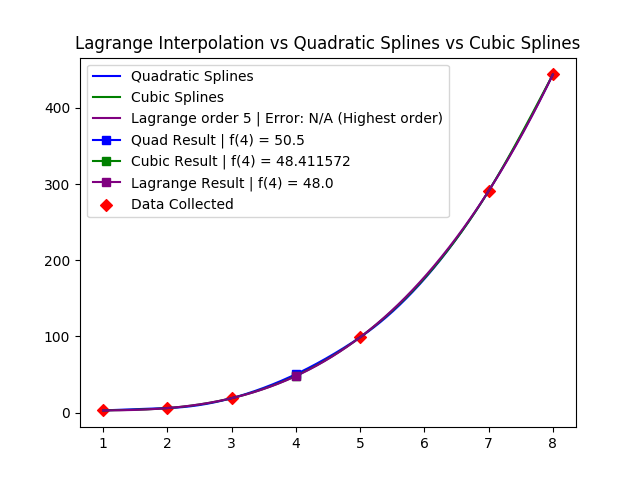
\includegraphics{Result0.png}
      \end{center}
  \part*{2/ Analyze and Comments}
    As the data given in Lab 7 is not good enough to demonstrate the differences between lagrange interpolation, quadratic spline, and
  cubic spline, I used the data given in the lesson's example and it clearly distinguished the curves. \\
    \begin{center}
      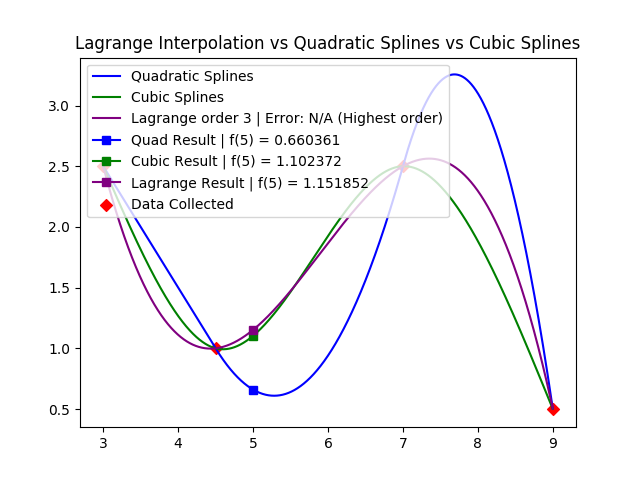
\includegraphics{Result1.png}
    \end{center}
    Overall, Lagrange interpolation gives us the best curve.
    The next closest curve is the curve created using cubic splines.
    The curve created with quadratic splines, in most cases, is not enough to describe the data accurately. \\
    In conclusion, we have to agree about 3 things:
    \begin{itemize}
      \item Newton and Lagrange interpolating polynomials better describe the data compared to splines in most cases,
      \item However, in cases when Newton and Lagrange does not work, splines could be used and it will give a fair enough result.
      \item The higher order of the polynomials, for both interpolation and splines, always guarantee us a more accurate model.
    \end{itemize}
  \end{document}